\documentclass[pdftex,titlepage]{article}

\author{Noah Santschi-Cooney - 116361061}
\title{Alternative Visualisation of Distributed Tracing data in a complex, large-scale distributed system}

\usepackage{graphicx}
\graphicspath{ {./assets/} }

\begin{document}
    \maketitle
    \section{Introduction}

    Modern Internet services are often implemented as complex, large-scale distributed systems. 
    These applications are constructed from collections of software modules that could span many
    thousands of machines across multiple physical facilities. With the rise of modern 
    Micro-service and Service-Oriented designs, traditional tooling used to monitor application 
    behaviour is no longer viable, especially at scale. To understanding the flow and lifecycle 
    of a unit of work performed in multiple pieces across various components in a distributed system, 
    the concept of Distributed Tracing was born. 
    Distributed Tracing was first introduced to the mainstream world in 2010 after the publication
    of Google’s Dapper paper. Since then, various vendors have come out with their own Dapper-inspired
    services, most of them based off flame or timeline graphs.

    \section{Distributed Tracing}
    The concept of Distributed Tracing has existed for over a decade at the time of writing. 
    This section will provide a brief history and overview of the concept and implementations of Distributed Tracing,
    from the first published paper of the implementation at Google to modern day standards.

        \subsection{Dapper}
        Released in April 2010,
        Google published a paper describing the design decisions behind an in-house implementation of distributed tracing,
        named Dapper. It is commonly believed that this paper describes the common ancestor to many tools that implement
        a form of distributed tracing.

        \paragraph{}
        The Dapper paper introduces some of the core primitives that underpin modern day standards. Most notable are the concepts
        of a \textit{trace tree} and its nodes, which are referred to as \textit{spans}. The trace tree forms a relationship between
        spans, not unakin to a stack trace, including however, continuing the analogy, stack frames over time, rather than just the 
        active stack frames at a certain point in time.
        
        \begin{figure}[htb!]
            \centering
            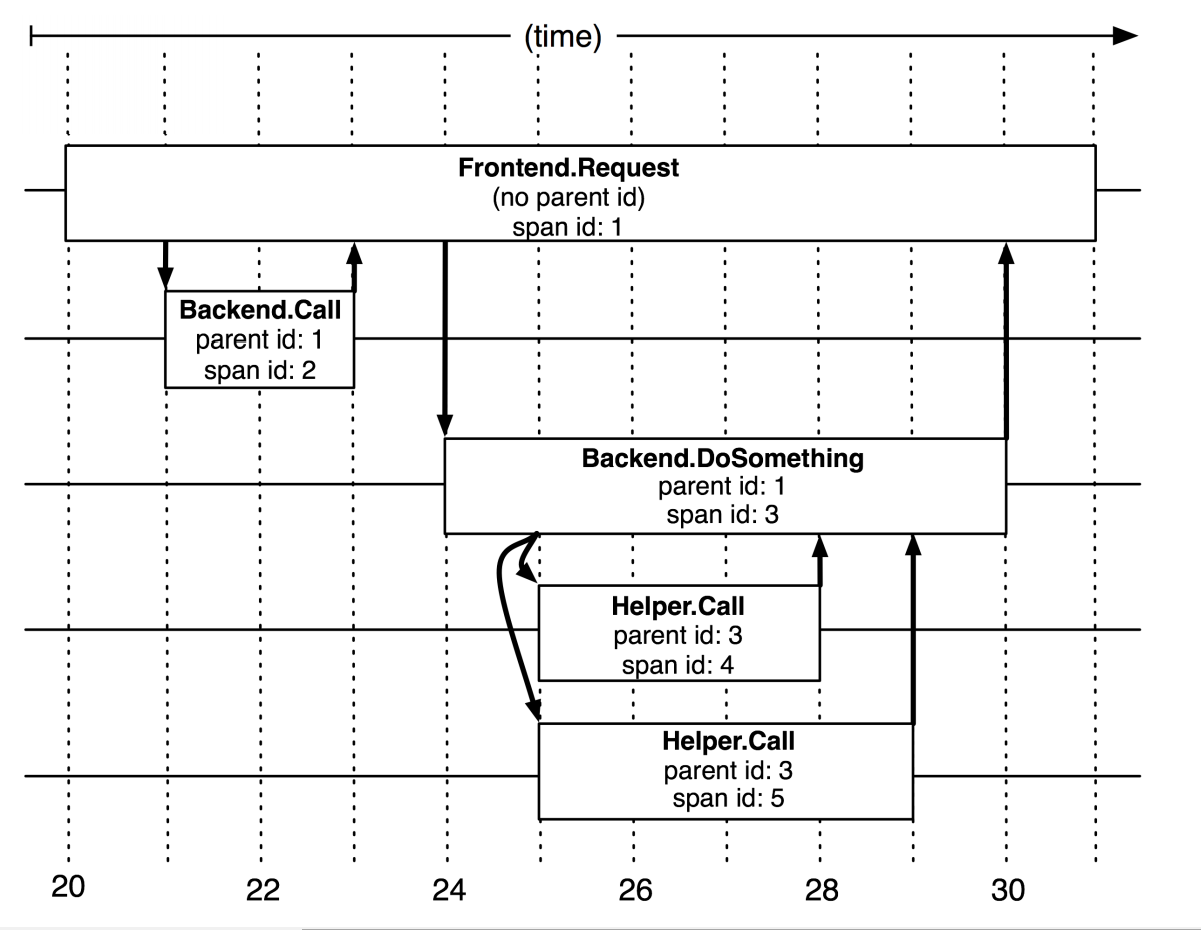
\includegraphics[scale=0.8]{dappertrace}
            \caption{The relationships between traces in a trace tree}
        \end{figure}


        \newpage


    \section{Main Chapter}

    \subsection{No}

    \section{Conclusion}
    
\end{document}